\documentclass[a4paper, 14pt]{extarticle}

% Поля
%--------------------------------------
\usepackage{geometry}
\geometry{a4paper,tmargin=2cm,bmargin=2cm,lmargin=3cm,rmargin=1cm}
%--------------------------------------


%Russian-specific packages
%--------------------------------------
\usepackage[T2A]{fontenc}
\usepackage[utf8]{inputenc} 
\usepackage[english, main=russian]{babel}
%--------------------------------------

\usepackage{textcomp}

% Красная строка
%--------------------------------------
\usepackage{indentfirst}               
%--------------------------------------             


%Graphics
%--------------------------------------
\usepackage{graphicx}
\graphicspath{ {./images/} }
\usepackage{wrapfig}
%--------------------------------------

% Полуторный интервал
%--------------------------------------
\linespread{1.3}                    
%--------------------------------------

%Выравнивание и переносы
%--------------------------------------
% Избавляемся от переполнений
\sloppy
% Запрещаем разрыв страницы после первой строки абзаца
\clubpenalty=10000
% Запрещаем разрыв страницы после последней строки абзаца
\widowpenalty=10000
%--------------------------------------

%Списки
\usepackage{enumitem}

%Подписи
\usepackage{caption} 

%Гиперссылки
\usepackage{hyperref}

\hypersetup {
	unicode=true
}

%Рисунки
%--------------------------------------
\DeclareCaptionLabelSeparator*{emdash}{~--- }
\captionsetup[figure]{labelsep=emdash,font=onehalfspacing,position=bottom}
%--------------------------------------

\usepackage{tempora}

%Листинги
%--------------------------------------
\usepackage{listings}
\lstset{
  basicstyle=\ttfamily\footnotesize, 
  %basicstyle=\footnotesize\AnkaCoder,        % the size of the fonts that are used for the code
  breakatwhitespace=false,         % sets if automatic breaks shoulbd only happen at whitespace
  breaklines=true,                 % sets automatic line breaking
  captionpos=t,                    % sets the caption-position to bottom
  inputencoding=utf8,
  frame=single,                    % adds a frame around the code
  keepspaces=true,                 % keeps spaces in text, useful for keeping indentation of code (possibly needs columns=flexible)
  keywordstyle=\bf,       % keyword style
  numbers=left,                    % where to put the line-numbers; possible values are (none, left, right)
  numbersep=5pt,                   % how far the line-numbers are from the code
  xleftmargin=25pt,
  xrightmargin=25pt,
  showspaces=false,                % show spaces everywhere adding particular underscores; it overrides 'showstringspaces'
  showstringspaces=false,          % underline spaces within strings only
  showtabs=false,                  % show tabs within strings adding particular underscores
  stepnumber=1,                    % the step between two line-numbers. If it's 1, each line will be numbered
  tabsize=2,                       % sets default tabsize to 8 spaces
  title=\lstname                   % show the filename of files included with \lstinputlisting; also try caption instead of title
}
%--------------------------------------

%%% Математические пакеты %%%
%--------------------------------------
\usepackage{amsthm,amsfonts,amsmath,amssymb,amscd}  % Математические дополнения от AMS
\usepackage{mathtools}                              % Добавляет окружение multlined
\usepackage[perpage]{footmisc}
%--------------------------------------

%--------------------------------------
%			НАЧАЛО ДОКУМЕНТА
%--------------------------------------

\begin{document}

%--------------------------------------
%			ТИТУЛЬНЫЙ ЛИСТ
%--------------------------------------
\begin{titlepage}
\thispagestyle{empty}
\newpage


%Шапка титульного листа
%--------------------------------------
\vspace*{-60pt}
\hspace{-65pt}
\begin{minipage}{0.3\textwidth}
\hspace*{-20pt}\centering

\includegraphics[width=\textwidth]{emblem}
\end{minipage}
\begin{minipage}{0.67\textwidth}\small \textbf{
\vspace*{-0.7ex}
\hspace*{-6pt}\centerline{Министерство науки и высшего образования Российской Федерации}
\vspace*{-0.7ex}
\centerline{Федеральное государственное бюджетное образовательное учреждение }
\vspace*{-0.7ex}
\centerline{высшего образования}
\vspace*{-0.7ex}
\centerline{<<Московский государственный технический университет}
\vspace*{-0.7ex}
\centerline{имени Н.Э. Баумана}
\vspace*{-0.7ex}
\centerline{(национальный исследовательский университет)>>}
\vspace*{-0.7ex}
\centerline{(МГТУ им. Н.Э. Баумана)}}
\end{minipage}
%--------------------------------------

%Полосы
%--------------------------------------
\vspace{-25pt}
\hspace{-35pt}\rule{\textwidth}{2.3pt}

\vspace*{-20.3pt}
\hspace{-35pt}\rule{\textwidth}{0.4pt}
%--------------------------------------

\vspace{1.5ex}
\hspace{-35pt} \noindent \small ФАКУЛЬТЕТ\hspace{80pt} <<Информатика и системы управления>>

\vspace*{-16pt}
\hspace{47pt}\rule{0.83\textwidth}{0.4pt}

\vspace{0.5ex}
\hspace{-35pt} \noindent \small КАФЕДРА\hspace{50pt} <<Теоретическая информатика и компьютерные технологии>>

\vspace*{-16pt}
\hspace{30pt}\rule{0.866\textwidth}{0.4pt}
  
\vspace{11em}

\begin{center}
\Large {\bf Лабораторная работа № 4} \\
\large {\bf по курсу <<Теория искусственных нейронных сетей>>} \\
\end{center}\normalsize

\vspace{8em}


\begin{flushright}
  {Студентка группы ИУ9-72Б Самохвалова П. С. \hspace*{15pt}\\
  \vspace{2ex}
  Преподаватель Каганов Ю. Т.\hspace*{15pt}}
\end{flushright}

\bigskip

\vfill
 

\begin{center}
\textsl{Москва 2023}
\end{center}
\end{titlepage}
%--------------------------------------
%		КОНЕЦ ТИТУЛЬНОГО ЛИСТА
%--------------------------------------

\renewcommand{\ttdefault}{pcr}

\setlength{\tabcolsep}{3pt}
\newpage
\setcounter{page}{2}

\section{Задание}\label{Sect::task}

\begin{enumerate}
    \item Сравнительный анализ современных методов оптимизации (SGD, NAG, Adagrad, Adam) на примере многослойного персептрона.
    \item Использование генетического алгоритма для оптимизации гиперпараметров (число слоев и число нейронов) многослойного персептрона.
\end{enumerate}

\section{Практическая реализация}\label{Sect::code}

Исходный код программы представлен в листинге~\ref{lst:code1}.

\begin{lstlisting}[language={python},caption={Методы оптимизации на примере многослойного персептрона, генетический алгоритм},label={lst:code1}]
import random
import pickle
import gzip
import numpy as np
from matplotlib import pyplot as plt


def load_data():
    with gzip.open('../data/mnist.pkl.gz', 'rb') as f:
        (training_data, validation_data, test_data) = pickle.load(f, encoding='latin1')
    return (training_data, validation_data, test_data)


def load_data_wrapper():
    tr_d, va_d, te_d = load_data()
    training_inputs = [np.reshape(x, (784, 1)) for x in tr_d[0]]
    training_results = [vectorized_result(y) for y in tr_d[1]]
    training_data = list(zip(training_inputs, training_results))
    validation_inputs = [np.reshape(x, (784, 1)) for x in va_d[0]]
    validation_data = list(zip(validation_inputs, va_d[1]))
    test_inputs = [np.reshape(x, (784, 1)) for x in te_d[0]]
    test_data = list(zip(test_inputs, te_d[1]))
    return (training_data, validation_data, test_data)


def vectorized_result(j):
    e = np.zeros((10, 1))
    e[j] = 1.0
    return e


def sigmoid(x):
    return 1 / (1 + np.exp(-x))


def sigmoid_der(x):
    return sigmoid(x) * (1 - sigmoid(x))


def relu(x):
    x = x.flatten()
    return np.array([[max(c, 0)] for c in x])


def relu_der(x):
    x = x.flatten()
    return np.array([[1 if c > 0 else 0] for c in x])


def softmax(z):
    e_z = np.exp(z - np.max(z))
    return e_z / e_z.sum()


def softmax_der(z):
    s = softmax(z)
    return np.diag(s) - np.outer(s, s)


def mse(y_true, y_received):
    return np.linalg.norm(y_true - y_received)


def mse_der(y_true, y_received):
    return y_true - y_received


def categorical_cross_entropy(y0, y):
    return -(y0 * np.log(y) + (1 - y0) * np.log(1 - y))


def categorical_cross_entropy_der(y0, y):
    return -(y0 / y - (1 - y0) / (1 - y))


def kl_divergence(y0, y):
    if y0 == 0:
        return 0
    else:
        return y0 * np.log(y0 / y)


def kl_divergence_der(y0, y):
    return np.log(y0 / y) + 1


class MultilayerPerceptron(object):

    def __init__(self, sizes, optimization_method, activation_function, loss_function):
        self.num_layers = len(sizes)
        self.optimization_method = optimization_method
        self.activation_function = activation_function
        if activation_function == sigmoid:
            self.activation_function_der = sigmoid_der
        elif activation_function == relu:
            self.activation_function_der = relu_der
        elif activation_function == softmax:
            self.activation_function_der = softmax_der
        self.loss_function = loss_function
        if loss_function == mse:
            self.loss_function_der = mse_der
        elif loss_function == categorical_cross_entropy:
            self.loss_function_der = categorical_cross_entropy_der
        elif self.loss_function == kl_divergence:
            self.loss_function_der = kl_divergence_der
        self.sizes = sizes
        self.biases = [np.random.randn(y, 1) for y in sizes[1:]]
        self.weights = [np.random.randn(y, x) for x, y in zip(sizes[:-1], sizes[1:])]
        self.loss = []
        if optimization_method == "adagrad":
            self.G_b = [np.zeros(b.shape) for b in self.biases]
            self.G_w = [np.zeros(w.shape) for w in self.weights]
        if self.optimization_method == "adam":
            self.beta1 = 0.9
            self.beta2 = 0.999
            self.epsilon = 1e-8
            self.m_w = [np.zeros(w.shape) for w in self.weights]
            self.v_w = [np.zeros(w.shape) for w in self.weights]
            self.m_b = [np.zeros(b.shape) for b in self.biases]
            self.v_b = [np.zeros(b.shape) for b in self.biases]
            self.t = 0
        if self.optimization_method == "nag":
            self.velocity_biases = [np.zeros(b.shape) for b in self.biases]
            self.velocity_weights = [np.zeros(w.shape) for w in self.weights]

    def feedforward(self, a):
        for b, w in zip(self.biases, self.weights):
            a = self.activation_function(np.dot(w, a) + b)
        return a

    def train(self, training_data, epochs, mini_batch_size, eta, test_data):
        if self.optimization_method == "sgd":
            self.SGD(training_data, epochs, mini_batch_size, eta, test_data)
        elif self.optimization_method == "adagrad":
            self.Adagrad(training_data, epochs, mini_batch_size, eta, test_data)
        elif self.optimization_method == "adam":
            self.Adam(training_data, epochs, mini_batch_size, eta, test_data)
        elif self.optimization_method == "nag":
            self.NAG(training_data, epochs, mini_batch_size, eta, test_data)

    def SGD(self, training_data, epochs, mini_batch_size, eta, test_data):
        n = len(training_data)
        for j in range(epochs):
            random.shuffle(training_data)
            mini_batches = [training_data[k : k+mini_batch_size] for k in range(0, n, mini_batch_size)]
            for mini_batch in mini_batches:
                self.update_mini_batch(mini_batch, eta)
            self.test(test_data)

    def update_mini_batch(self, mini_batch, eta):
        nabla_b = [np.zeros(b.shape) for b in self.biases]
        nabla_w = [np.zeros(w.shape) for w in self.weights]
        for x, y in mini_batch:
            delta_nabla_b, delta_nabla_w = self.backprop(x, y)
            nabla_b = [nb + dnb for nb, dnb in zip(nabla_b, delta_nabla_b)]
            nabla_w = [nw + dnw for nw, dnw in zip(nabla_w, delta_nabla_w)]
        self.weights = [w - (eta / len(mini_batch)) * nw for w, nw in zip(self.weights, nabla_w)]
        self.biases = [b - (eta / len(mini_batch)) * nb for b, nb in zip(self.biases, nabla_b)]

    def backprop(self, x, y):
        nabla_b = [np.zeros(b.shape) for b in self.biases]
        nabla_w = [np.zeros(w.shape) for w in self.weights]

        activation = x
        activations = [x]
        zs = []
        for b, w in zip(self.biases, self.weights):
            z = np.dot(w, activation) + b
            zs.append(z)
            activation = self.activation_function(z)
            activations.append(activation)

        delta = self.loss_function_der(activations[-1], y) * self.activation_function_der(zs[-1])
        nabla_b[-1] = delta
        nabla_w[-1] = np.dot(delta, activations[-2].transpose())

        for l in range(2, self.num_layers):
            z = zs[-l]
            sp = self.activation_function_der(z)
            delta = np.dot(self.weights[-l + 1].transpose(), delta) * sp
            nabla_b[-l] = delta
            nabla_w[-l] = np.dot(delta, activations[-l - 1].transpose())

        return (nabla_b, nabla_w)

    def Adagrad(self, training_data, epochs, mini_batch_size, eta, test_data):
        n = len(training_data)
        for j in range(epochs):
            random.shuffle(training_data)
            mini_batches = [training_data[k: k + mini_batch_size] for k in range(0, n, mini_batch_size)]
            for mini_batch in mini_batches:
                self.update_mini_batch_adagrad(mini_batch, eta)
            self.test(test_data)

    def update_mini_batch_adagrad(self, mini_batch, eta):
        epsilon = 1e-8
        for x, y in mini_batch:
            nabla_b, nabla_w = self.backprop(x, y)
            for l in range(self.num_layers - 1):
                self.G_b[l] += nabla_b[l] ** 2
                self.G_w[l] += nabla_w[l] ** 2
            for l in range(self.num_layers - 1):
                self.biases[l] -= (eta / (np.sqrt(self.G_b[l] + epsilon))) * nabla_b[l]
                self.weights[l] -= (eta / (np.sqrt(self.G_w[l] + epsilon))) * nabla_w[l]

    def Adam(self, training_data, epochs, mini_batch_size, eta, test_data):
        n = len(training_data)
        for j in range(epochs):
            random.shuffle(training_data)
            mini_batches = [training_data[k: k + mini_batch_size] for k in range(0, n, mini_batch_size)]
            for mini_batch in mini_batches:
                self.update_mini_batch_adam(mini_batch, eta)
            self.test(test_data)

    def update_mini_batch_adam(self, mini_batch, eta):
        self.t += 1

        for x, y in mini_batch:
            delta_nabla_b, delta_nabla_w = self.backprop(x, y)
            self.m_w = [(self.beta1 * mw + (1 - self.beta1) * dw) for mw, dw in zip(self.m_w, delta_nabla_w)]
            self.v_w = [(self.beta2 * vw + (1 - self.beta2) * (dw ** 2)) for vw, dw in zip(self.v_w, delta_nabla_w)]
            self.m_b = [(self.beta1 * mb + (1 - self.beta1) * db) for mb, db in zip(self.m_b, delta_nabla_b)]
            self.v_b = [(self.beta2 * vb + (1 - self.beta2) * (db ** 2)) for vb, db in zip(self.v_b, delta_nabla_b)]

        m_w_corrected = [mw / (1 - self.beta1 ** self.t) for mw in self.m_w]
        v_w_corrected = [vw / (1 - self.beta2 ** self.t) for vw in self.v_w]
        m_b_corrected = [mb / (1 - self.beta1 ** self.t) for mb in self.m_b]
        v_b_corrected = [vb / (1 - self.beta2 ** self.t) for vb in self.v_b]

        self.weights = [w - (eta / (np.sqrt(vw) + self.epsilon)) * mw_corr for w, vw, mw_corr in zip(self.weights, v_w_corrected, m_w_corrected)]
        self.biases = [b - (eta / (np.sqrt(vb) + self.epsilon)) * mb_corr for b, vb, mb_corr in zip(self.biases, v_b_corrected, m_b_corrected)]

    def NAG(self, training_data, epochs, mini_batch_size, eta, test_data):
        n = len(training_data)
        for j in range(epochs):
            random.shuffle(training_data)
            mini_batches = [training_data[k : k+mini_batch_size] for k in range(0, n, mini_batch_size)]
            for mini_batch in mini_batches:
                self.update_mini_batch_nag(mini_batch, eta)
            self.test(test_data)

    def update_mini_batch_nag(self, mini_batch, eta, gamma=0.9):
        nabla_b = [np.zeros(b.shape) for b in self.biases]
        nabla_w = [np.zeros(w.shape) for w in self.weights]
        for x, y in mini_batch:
            delta_nabla_b, delta_nabla_w = self.backprop(x, y)
            nabla_b = [nb + dnb for nb, dnb in zip(nabla_b, delta_nabla_b)]
            nabla_w = [nw + dnw for nw, dnw in zip(nabla_w, delta_nabla_w)]

        self.velocity_biases = [gamma * vb + (eta / len(mini_batch)) * nb for vb, nb in zip(self.velocity_biases, nabla_b)]
        self.velocity_weights = [gamma * vw + (eta / len(mini_batch)) * nw for vw, nw in zip(self.velocity_weights, nabla_w)]

        self.weights = [w - vw for w, vw in zip(self.weights, self.velocity_weights)]
        self.biases = [b - vb for b, vb in zip(self.biases, self.velocity_biases)]

    def test(self, test_data):
        n_test = len(test_data)
        s = 0
        for i in range(n_test):
            y_receivied = self.feedforward(test_data[i][0])
            y_true = vectorized_result(test_data[i][1])
            s += self.loss_function(y_true, y_receivied)
        s /= n_test
        self.loss.append(s)

    def get_loss(self, i):
        return self.loss[i]

    def recognize(self, test_example):
        return np.argmax(self.feedforward(test_example))


def genetic_algorithm(Mp, Np, f):

    population = [[random.uniform(0, 1), random.randint(1, 10)] for _ in range(Mp)]

    for k in range(Np):
        fitness = [1 / f(population[i]) for i in range(Mp)]
        fit = sum(fitness)
        p = [0] * Mp
        for i in range(Mp):
            for j in range(i + 1):
                p[i] += fitness[j] / fit
        p = [0] + p
        cross = []
        for i in range(Mp):
            r = random.uniform(1e-7, 1.0)
            for j in range(1, Mp + 1):
                if p[j - 1] < r <= p[j]:
                    cross.append(population[j - 1])
        population_n = []
        for i in range(Mp):
            r = random.uniform(1e-7, 1 - 1e-7)
            new_fraction = r * cross[i][0] + (1 - r) * cross[i][1]
            new_integer = random.randint(1, 10)
            population_n.append([new_fraction, new_integer])
        pm = random.uniform(0.05, 0.2)
        mutations = []
        for i in range(Mp):
            r = random.uniform(0, 1)
            if r < pm:
                mutations.append(population_n[i])
        for i in range(len(mutations)):
            index = random.randint(0, 1)
            if index == 0:
                mutations[i][0] = random.uniform(0, 1)
            else:
                mutations[i][1] = random.randint(1, 10)
        if len(mutations) > 0:
            fitness = [1 / f(population_n[i]) for i in range(Mp)]
            min_fitness_idx = np.argmin(fitness)
            population_n[min_fitness_idx] = mutations[random.randint(0, len(mutations) - 1)]
        for i in range(Mp):
            population[i] = population_n[i]

    fitness = [1 / f(population[i]) for i in range(Mp)]
    max_fitness_idx = np.argmax(fitness)
    print("Genetic algorithm")
    print(population[max_fitness_idx])


def function(x):
    global training_data, test_data
    eta = x[0]
    num_neurons = x[1]
    epochs = 2
    perceptron = MultilayerPerceptron([784, num_neurons, 10], "sgd", sigmoid, mse)
    perceptron.train(training_data, epochs, 10, eta, test_data)
    return perceptron.get_loss(epochs - 1)


epochs = 100
eta = 0.01


training_data, validation_data, test_data = load_data_wrapper()

perceptron = MultilayerPerceptron([784, 8, 10], "sgd", sigmoid, mse)

perceptron.train(training_data, epochs, 10, eta, test_data)

print(perceptron.weights)

plt.plot([i for i in range(epochs)], [perceptron.get_loss(i) for i in range(epochs)], label='SGD', color='blue')
plt.xlabel('Epochs')
plt.ylabel('Loss')
plt.title('Loss and Epochs')
plt.legend()
plt.show()

print()
for i in range(5):
    print("Expected:", test_data[i][1])
    print("Receivied:", perceptron.recognize(test_data[i][0]))
    print()


# training_data, validation_data, test_data = load_data_wrapper()
#
# perceptron = MultilayerPerceptron([784, 8, 10], "adagrad", sigmoid, mse)
#
# perceptron.train(training_data, epochs, 10, eta, test_data)
#
# print(perceptron.weights)
#
# plt.plot([i for i in range(epochs)], [perceptron.get_loss(i) for i in range(epochs)], label='Adagrad', color='red')
# plt.xlabel('Epochs')
# plt.ylabel('Loss')
# plt.title('Loss and Epochs')
# plt.legend()
# plt.show()
#
# print()
# for i in range(5):
#     print("Expected:", test_data[i][1])
#     print("Receivied:", perceptron.recognize(test_data[i][0]))
#     print()


# training_data, validation_data, test_data = load_data_wrapper()
#
# perceptron = MultilayerPerceptron([784, 8, 10], "adam", sigmoid, mse)
#
# perceptron.train(training_data, epochs, 10, eta, test_data)
#
# print(perceptron.weights)
#
# plt.plot([i for i in range(epochs)], [perceptron.get_loss(i) for i in range(epochs)], label='Adam', color='green')
# plt.xlabel('Epochs')
# plt.ylabel('Loss')
# plt.title('Loss and Epochs')
# plt.legend()
# plt.show()
#
# print()
# for i in range(5):
#     print("Expected:", test_data[i][1])
#     print("Receivied:", perceptron.recognize(test_data[i][0]))
#     print()


# training_data, validation_data, test_data = load_data_wrapper()
#
# perceptron = MultilayerPerceptron([784, 8, 10], "nag", sigmoid, mse)
#
# perceptron.train(training_data, epochs, 10, eta, test_data)
#
# print(perceptron.weights)
#
# plt.plot([i for i in range(epochs)], [perceptron.get_loss(i) for i in range(epochs)], label='NAG', color='brown')
# plt.xlabel('Epochs')
# plt.ylabel('Loss')
# plt.title('Loss and Epochs')
# plt.legend()
# plt.show()
#
# print()
# for i in range(5):
#     print("Expected:", test_data[i][1])
#     print("Receivied:", perceptron.recognize(test_data[i][0]))
#     print()


# Mp = 3
# Np = 5
#
# training_data, validation_data, test_data = load_data_wrapper()
#
# genetic_algorithm(Mp, Np, function)


\end{lstlisting}

\section{Результаты}\label{Sect::res}

Результаты работы программы представлены на рисунках~\ref{fig:img1}-~\ref{fig:img2}.

\begin{figure}[!htb]
	\centering
	
\includegraphics[width=0.8\textwidth]{img1}
\caption{Результат работы методов оптимизации SGD, Adagrad, Adam, NAG для многослойного персептрона}
\label{fig:img1}
\end{figure}

\begin{figure}[!htb]
	\centering
	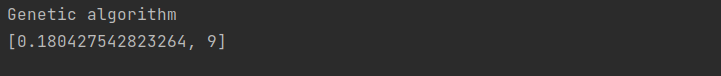
\includegraphics[width=0.8\textwidth]{img2}
\caption{Результат работы генетического алгоритма для оптимизации гиперпараметров многослойного персептрона}
\label{fig:img2}
\end{figure}

\section{Выводы}\label{Sect::conclusion}

В результате выполнения лабораторной работы были реализованы методы оптимизации SGD, Adagrad, Adam, NAG для многослойного персептрона, был реализован генетический алгоритм для оптимизации гиперпараметров многослойного персептрона.

\end{document}
